\documentclass[a4paper,twoside,10pt]{book}
% PAGE DIMENSIONS
% FOR A5 without scaling
%\usepackage[inner=18mm, outer=10mm,top=20mm,headsep=10mm,bottom=10mm,paperwidth=148mm,paperheight=210mm]{geometry}
% FOR 17x24cm
\usepackage[inner=30mm, outer=20mm,top=24mm,headsep=10mm,bottom=20mm,paperwidth=170mm,paperheight=240mm]{geometry}
% FOR A4
%\usepackage[inner=50mm, outer=40mm,top=60mm,headsep=10mm,bottom=57mm,paperwidth=210mm,paperheight=297mm]{geometry}
%\usepackage[inner=8.5mm, outer=12.5mm,top=10mm,headsep=5mm,bottom=10mm,paperwidth=141mm,paperheight=200mm]{geometry}
%\usepackage[inner=30mm, outer=23mm,top=29mm,headsep=10mm,bottom=23mm,paperwidth=210mm,paperheight=297mm]{geometry}
% FOR A5
%\usepackage[inner=25mm, outer=17mm,top=8mm,headsep=8mm,bottom=17mm,paperwidth=148mm,paperheight=210mm,includehead]{geometry}
% TABLES: full-width using X{10cm} column
\usepackage{tabularx}
% DRAWINGS (for chapter title)
\usepackage{tikz}
% TYPOGRAPHY: 
\usepackage[protrusion=true,final,factor=1500]{microtype}

% SOME extra math symbols
\usepackage{amssymb}




% CAPTIONS of figures/table styling
\usepackage[font={stretch=1.1,small},labelfont=bf]{caption} % order matters: stretch, then size
%\usepackage[font={small,sf},labelfont=bf]{caption} % small sans-serif + bold

% FONT  SIZES
\usepackage{fix-cm} % FOR ANY font sizes, not predefined
\renewcommand\footnotesize{\fontsize{7pt}{7pt}\selectfont}
\renewcommand\small{\fontsize{6pt}{6pt}\selectfont}
\renewcommand\normalsize{\fontsize{9pt}{9pt}\selectfont}
\renewcommand\large{\fontsize{10pt}{10pt}\selectfont}
\renewcommand\Large{\fontsize{11pt}{11pt}\selectfont}
\renewcommand\Huge{\fontsize{24pt}{24pt}\selectfont}

% LINE spacing
\renewcommand{\baselinestretch}{1.25}

% FONTS for LaTeX/XeLaTeX
\usepackage{ifxetex}
\ifxetex
			\usepackage{mathspec}
			\usepackage{polyglossia}
			\setdefaultlanguage[variant=uk]{english}
			\defaultfontfeatures{Ligatures=TeX} % To support LaTeX quoting style
			\setmainfont{Minion Pro} 
			\setsansfont{Myriad Pro}
			\setmathsfont(Digits,Greek,Latin)[Numbers={Proportional}]{Minion Pro}
			\setmathrm{Minion Pro}
			\usepackage[italic]{mathastext}
			%\setmainfont[BoldFont={SwiftNeueLTW01-Bold},ItalicFont={SwiftNeueLTW01-Italic}]{SwiftNeueLTW01} 
			%\setsansfont{UniversLTW01-55Roman}
\else
			%\usepackage[T1]{fontenc}
			%\usepackage[utf8]{inputenc}
			\usepackage[english]{babel}
			%\usepackage{fouriernc} % UTOPIA + FOURIER
			%\usepackage{mathpple} % palatino
			%\usepackage[sc]{mathpazo}
			\usepackage[charter]{mathdesign} %utopia, garamond
			\usepackage[scaled]{helvet}
			%\usepackage{newtxtt}
			\def\ttdefault{cmvtt}
			%\usepackage[light]{roboto}
			%\renewcommand{\sfdefault}{ua1}
\fi

\usepackage{hyperref}
% HEADER/FOOTER
\usepackage{fancyhdr}
\renewcommand{\headrulewidth}{0pt}
\renewcommand{\footrulewidth}{0pt}
\fancyhf{}
\makeatletter
	\let\ps@plain\ps@empty
\makeatother
% PLAIN: for first page of chapter
\fancypagestyle{plain}{
	\renewcommand{\headrulewidth}{0pt}
	\fancyhf{}
	\fancyhead[RO]{
		\makebox[2cm][l]{
			\makebox[4cm][c]{\normalsize
				\hskip0.25em\phantom{\thepage}\phantom{XX}~~$\left|\vphantom{\int_a^b}\right.$~~\thepage\phantom{XX}
			}
		}
	}
	\fancyhead[LE]{
		\makebox[2cm][r]{
			\makebox[4cm][c]{\normalsize
				\hskip0.45em\phantom{XX}\thepage~~$\left|\vphantom{\int_a^b}\right.$~~\phantom{XX}\phantom{\thepage}
			}
		}
	}
}
% REGULAR pages
\fancyhead[RO]{
	\makebox[2cm][l]{
		\makebox[4cm][c]{\normalsize
			\hskip0.25em\phantom{\thepage}\nouppercase\rightmark~~$\left|\vphantom{\int_a^b}\right.$~~\thepage\phantom{\nouppercase\rightmark}
		}
	}
}
\fancyhead[LE]{
	\makebox[2cm][r]{
		\makebox[4cm][c]{\normalsize
			\hskip0.45em\phantom{\nouppercase\leftmark}\thepage~~$\left|\vphantom{\int_a^b}\right.$~~\nouppercase\leftmark\phantom{\thepage}
		}
	}
}

% MARGIN labels, except chapter=0 (intro; conclusion; bibliography etc.)
% AND \setcouter{chapter}{0} has to be set explicitely in required chapters
\fancyfoot[RO]{
	\ifnum\value{chapter}>0
	\begin{tikzpicture}[remember picture, overlay]
	\node[rounded corners=2mm,inner sep=3mm,anchor=north east,black,fill=black!15,draw=black!75] at ([xshift=2mm,yshift=-\arabic{chapter}*1.3cm-1.1cm]current page.north east) {\fontsize{1cm}{1cm}\selectfont\thechapter};
	\end{tikzpicture}
	\fi
}
\fancyfoot[LE]{
	\ifnum\value{chapter}>0
	\begin{tikzpicture}[remember picture, overlay]
	\node[rounded corners=2mm,inner sep=3mm,anchor=north west,black,fill=black!15,draw=black!75] at ([xshift=-2mm,yshift=-\arabic{chapter}*1.3cm-1.1cm]current page.north west) {\fontsize{1cm}{1cm}\selectfont\thechapter};
	\end{tikzpicture}
	\fi
}



\pagestyle{fancy}
% HEADER contents - chapter name and section name
%\renewcommand{\chaptermark}[1]{\markboth{\thechapter.\, #1}{}}
\renewcommand{\chaptermark}[1]{\markboth{#1}{}}
\renewcommand{\sectionmark}[1]{\markright{\thesection.\, #1}}


% FLOATING objects
\usepackage{float}
% PICTURES
\usepackage{graphicx}
% NOT USED
\usepackage{setspace}

% SPACINGS in lists
\usepackage{enumitem}
% VERICAL: topsep partopsep parsep itemsep
% HORIZONTAL: leftmargin rightmargin listparindent labelwidth labelsep itemindent
% GLOBAL: \setlist[enumerate]{labelsep=*, leftmargin=1.5pc}
%\setlist{noitemsep}
\setlist{nosep}




% TABLES: nicer rulers
% AND nicer spacing between lines in tables
\usepackage{booktabs}
\renewcommand{\arraystretch}{1.2}


% TITLES styling
\usepackage[toctitles,explicit,raggedright]{titlesec}
\newcommand*\chapterlabel{}
% CHAPTER in frontmatter|backmatter
\titleformat{name=\chapter,numberless}[display]
	{\normalfont\rmfamily\Huge\bfseries}{}{1ex}
	{\flushright{\chapterlabel#1}}
% CHAPTER in mainmatter
\titleformat{\chapter}
{\gdef\chapterlabel{}\normalfont\rmfamily\Huge\bfseries}
{\gdef\chapterlabel{}}{-10em}
{
	\flushright{
		\begin{tikzpicture}
			%\draw[help lines,step=5mm] (0,-3) grid (-\linewidth,3);
			\node[black!50,anchor=east,inner sep=0mm] (a) at (0,0) {\fontsize{7cm}{8cm}\selectfont\thechapter};
			\begin{scope}[cm={1,0,-0.6,0.15,(0,0)}].
					\node[transform shape,black!30,anchor=south,inner sep=0mm] at (a.south) {\fontsize{7cm}{8cm}\selectfont{}\thechapter};
					%\node[transform shape,black!30,anchor=south east,inner sep=0mm] at (a.south) {\fontsize{3cm}{8cm}\selectfont{}\chaptername};
			\end{scope}
			\node[black!50,anchor=east,inner sep=0mm] (a) at (0,0) {\fontsize{7cm}{8cm}\selectfont\thechapter};
			\node[black!35,anchor=east,inner sep=0.20mm,scale=0.98] at (0,0) {\fontsize{7cm}{8cm}\selectfont\thechapter};
			\node[black!20,anchor=east,inner sep=0.40mm,scale=0.96] at (0,0) {\fontsize{7cm}{8cm}\selectfont\thechapter};
			%\node[black!20,scale=0.97] at (a) {\fontsize{6cm}{8cm}\selectfont\thechapter};
			%\node[anchor=east,black!45] at (0,-1) {\resizebox{\linewidth}{!}{\chaptername}};
			%\node[anchor=north east,inner sep=0mm] at (a.north east) {\parbox{\linewidth}{\raggedleft\chapterlabel#1}};
			\node[anchor=east,inner sep=0mm] at (0,0) {\parbox{\linewidth}{\raggedleft\chapterlabel#1}};
		\end{tikzpicture}
		%\chapterlabel#1
	}
}
% SPACING: chapter by default uses \@makechapterhead with extra spacing before and after the chapter title
\titlespacing*{\chapter}{0pt}{-25pt}{30pt}

%\titleformat{\section}[block]{\Large}{\bfseries\thesection.\,\,#1}{1em}{}
%\titleformat{\subsection}[block]{\large}{\bfseries\thesubsection.\,\,#1}{1em}{}
%\titleformat{\subsection}{\no}{\itshape\thesubsection.\,#1}{1em}{}


% GREEK letters in section/chapter titles AND in PDF bookmarks
%\usepackage[artemisia]{textgreek}




\usepackage{listings}
\definecolor{mygreen}{rgb}{0,0.6,0}
\definecolor{mygray}{rgb}{0.5,0.5,0.5}
\definecolor{mymauve}{rgb}{0.58,0,0.82}
\usepackage{amsmath}
\usepackage{pgfplots}

\lstset{ 
	backgroundcolor=\color{white},   % choose the background color; you must add \usepackage{color} or \usepackage{xcolor}; should come as last argument
	basicstyle=\small\ttfamily,
	belowcaptionskip=0em,        % the size of the fonts that are used for the code
	belowskip=-2em,
	breakatwhitespace=false,         % sets if automatic breaks should only happen at whitespace
	breaklines=true,                 % sets automatic line breaking
	captionpos=b,                    % sets the caption-position to bottom
	commentstyle=\color{mygreen},    % comment style
	deletekeywords={...},            % if you want to delete keywords from the given language
	escapeinside={\%*}{*)},          % if you want to add LaTeX within your code
	extendedchars=true,              % lets you use non-ASCII characters; for 8-bits encodings only, does not work with UTF-8
	frame=single,	                   % adds a frame around the code
	keepspaces=true,                 % keeps spaces in text, useful for keeping indentation of code (possibly needs columns=flexible)
	keywordstyle=\color{blue},       % keyword style
	language=Python,                 % the language of the code
	morekeywords={*,...},            % if you want to add more keywords to the set
	numbers=none,                    % where to put the line-numbers; possible values are (none, left, right)
	numbersep=5pt,                   % how far the line-numbers are from the code
	numberstyle=\tiny\color{mygray}, % the style that is used for the line-numbers
	rulecolor=\color{black},         % if not set, the frame-color may be changed on line-breaks within not-black text (e.g. comments (green here))
	showspaces=false,                % show spaces everywhere adding particular underscores; it overrides 'showstringspaces'
	showstringspaces=false,          % underline spaces within strings only
	showtabs=false,                  % show tabs within strings adding particular underscores
	stepnumber=2,                    % the step between two line-numbers. If it's 1, each line will be numbered
	stringstyle=\color{mymauve},     % string literal style
	tabsize=2,	                   % sets default tabsize to 2 spaces
	title=\lstname 			          % show the filename of files included with \lstinputlisting; also try caption instead of title
}
\def\inline{\lstinline[basicstyle=\ttfamily,keywordstyle={}]} %https://tex.stackexchange.com/questions/44702/can-you-change-lstinline-without-changing-the-global-lstset

% https://tex.stackexchange.com/questions/31085/is-there-a-standard-way-to-title-a-list-of-bullets
% name is purpose
\newenvironment{exercize}[1]{%
\vspace{0.2em}\noindent{\Large\textbf{#1}}
	\begin{itemize}}
	{\end{itemize}}
\begin{document}
\chapter{Improving the way neural networks learn}
When a golf player is first learning to play golf, they usually spend most of their time developing a basic swing. Only gradually do they develop other shots, learning to chip, draw and fade the ball, building on and modifying their basic swing. In a similar way, up to now we've focused on understanding the backpropagation algorithm. It's our ``basic swing'', the foundation for learning in most work on neural networks. In this chapter I explain a suite of techniques which can be used to improve on our vanilla implementation of backpropagation, and so improve the way our networks learn.

The techniques we'll develop in this chapter include: a better choice of cost function, known as the cross-entropy cost function; four so-called ``regularization'' methods (L1 and L2 regularization, dropout, and artificial expansion of the training data), which make our networks better at generalizing beyond the training data; a better method for initializing the weights in the network; and a set of heuristics to help choose good hyper-parameters for the network. I'll also overview several other techniques in less depth. The discussions are largely independent of one another, and so you may jump ahead if you wish. We'll also implement many of the techniques in running code, and use them to improve the results obtained on the handwriting classification problem studied in Chapter 1.

Of course, we're only covering a few of the many, many techniques which have been developed for use in neural nets. The philosophy is that the best entree to the plethora of available techniques is in-depth study of a few of the most important. Mastering those important techniques is not just useful in its own right, but will also deepen your understanding of what problems can arise when you use neural networks. That will leave you well prepared to quickly pick up other techniques, as you need them.

\section{The cross-entropy cost function}
Most of us find it unpleasant to be wrong. Soon after beginning to learn the piano I gave my first performance before an audience. I was nervous, and began playing the piece an octave too low. I got confused, and couldn't continue until someone pointed out my error. I was very embarrassed. Yet while unpleasant, we also learn quickly when we're decisively wrong. You can bet that the next time I played before an audience I played in the correct octave! By contrast, we learn more slowly when our errors are less well-defined.

Ideally, we hope and expect that our neural networks will learn fast from their errors. Is this what happens in practice? To answer this question, let's look at a toy example. The example involves a neuron with just one input:

\begin{center}
	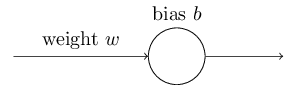
\includegraphics[width=0.5\linewidth]{figures/ch3/tikz28}
\end{center}
We'll train this neuron to do something ridiculously easy: take the input 1 to the output 0. Of course, this is such a trivial task that we could easily figure out an appropriate weight and bias by hand, without using a learning algorithm. However, it turns out to be illuminating to use gradient descent to attempt to learn a weight and bias. So let's take a look at how the neuron learns.

To make things definite, I'll pick the initial weight to be 0.6 and the initial bias to be 0.9. These are generic choices used as a place to begin learning, I wasn't picking them to be special in any way. The initial output from the neuron is 0.82, so quite a bit of learning will be needed before our neuron gets near the desired output, 0.0. 
%Click on ``Run'' in the bottom right corner below to see how the neuron learns an output much closer to 0.0. Note that this isn't a pre-recorded animation, your browser is actually computing the gradient, then using the gradient to update the weight and bias, and displaying the result.
The learning rate is $\eta$=0.15, which turns out to be slow enough that we can follow what's happening, but fast enough that we can get substantial learning in just a few seconds. The cost is the quadratic cost function, $C$, introduced back in Chapter 1. I'll remind you of the exact form of the cost function shortly, so there's no need to go and dig up the definition. %Note that you can run the animation multiple times by clicking on ``Run'' again.
\begin{center}%
	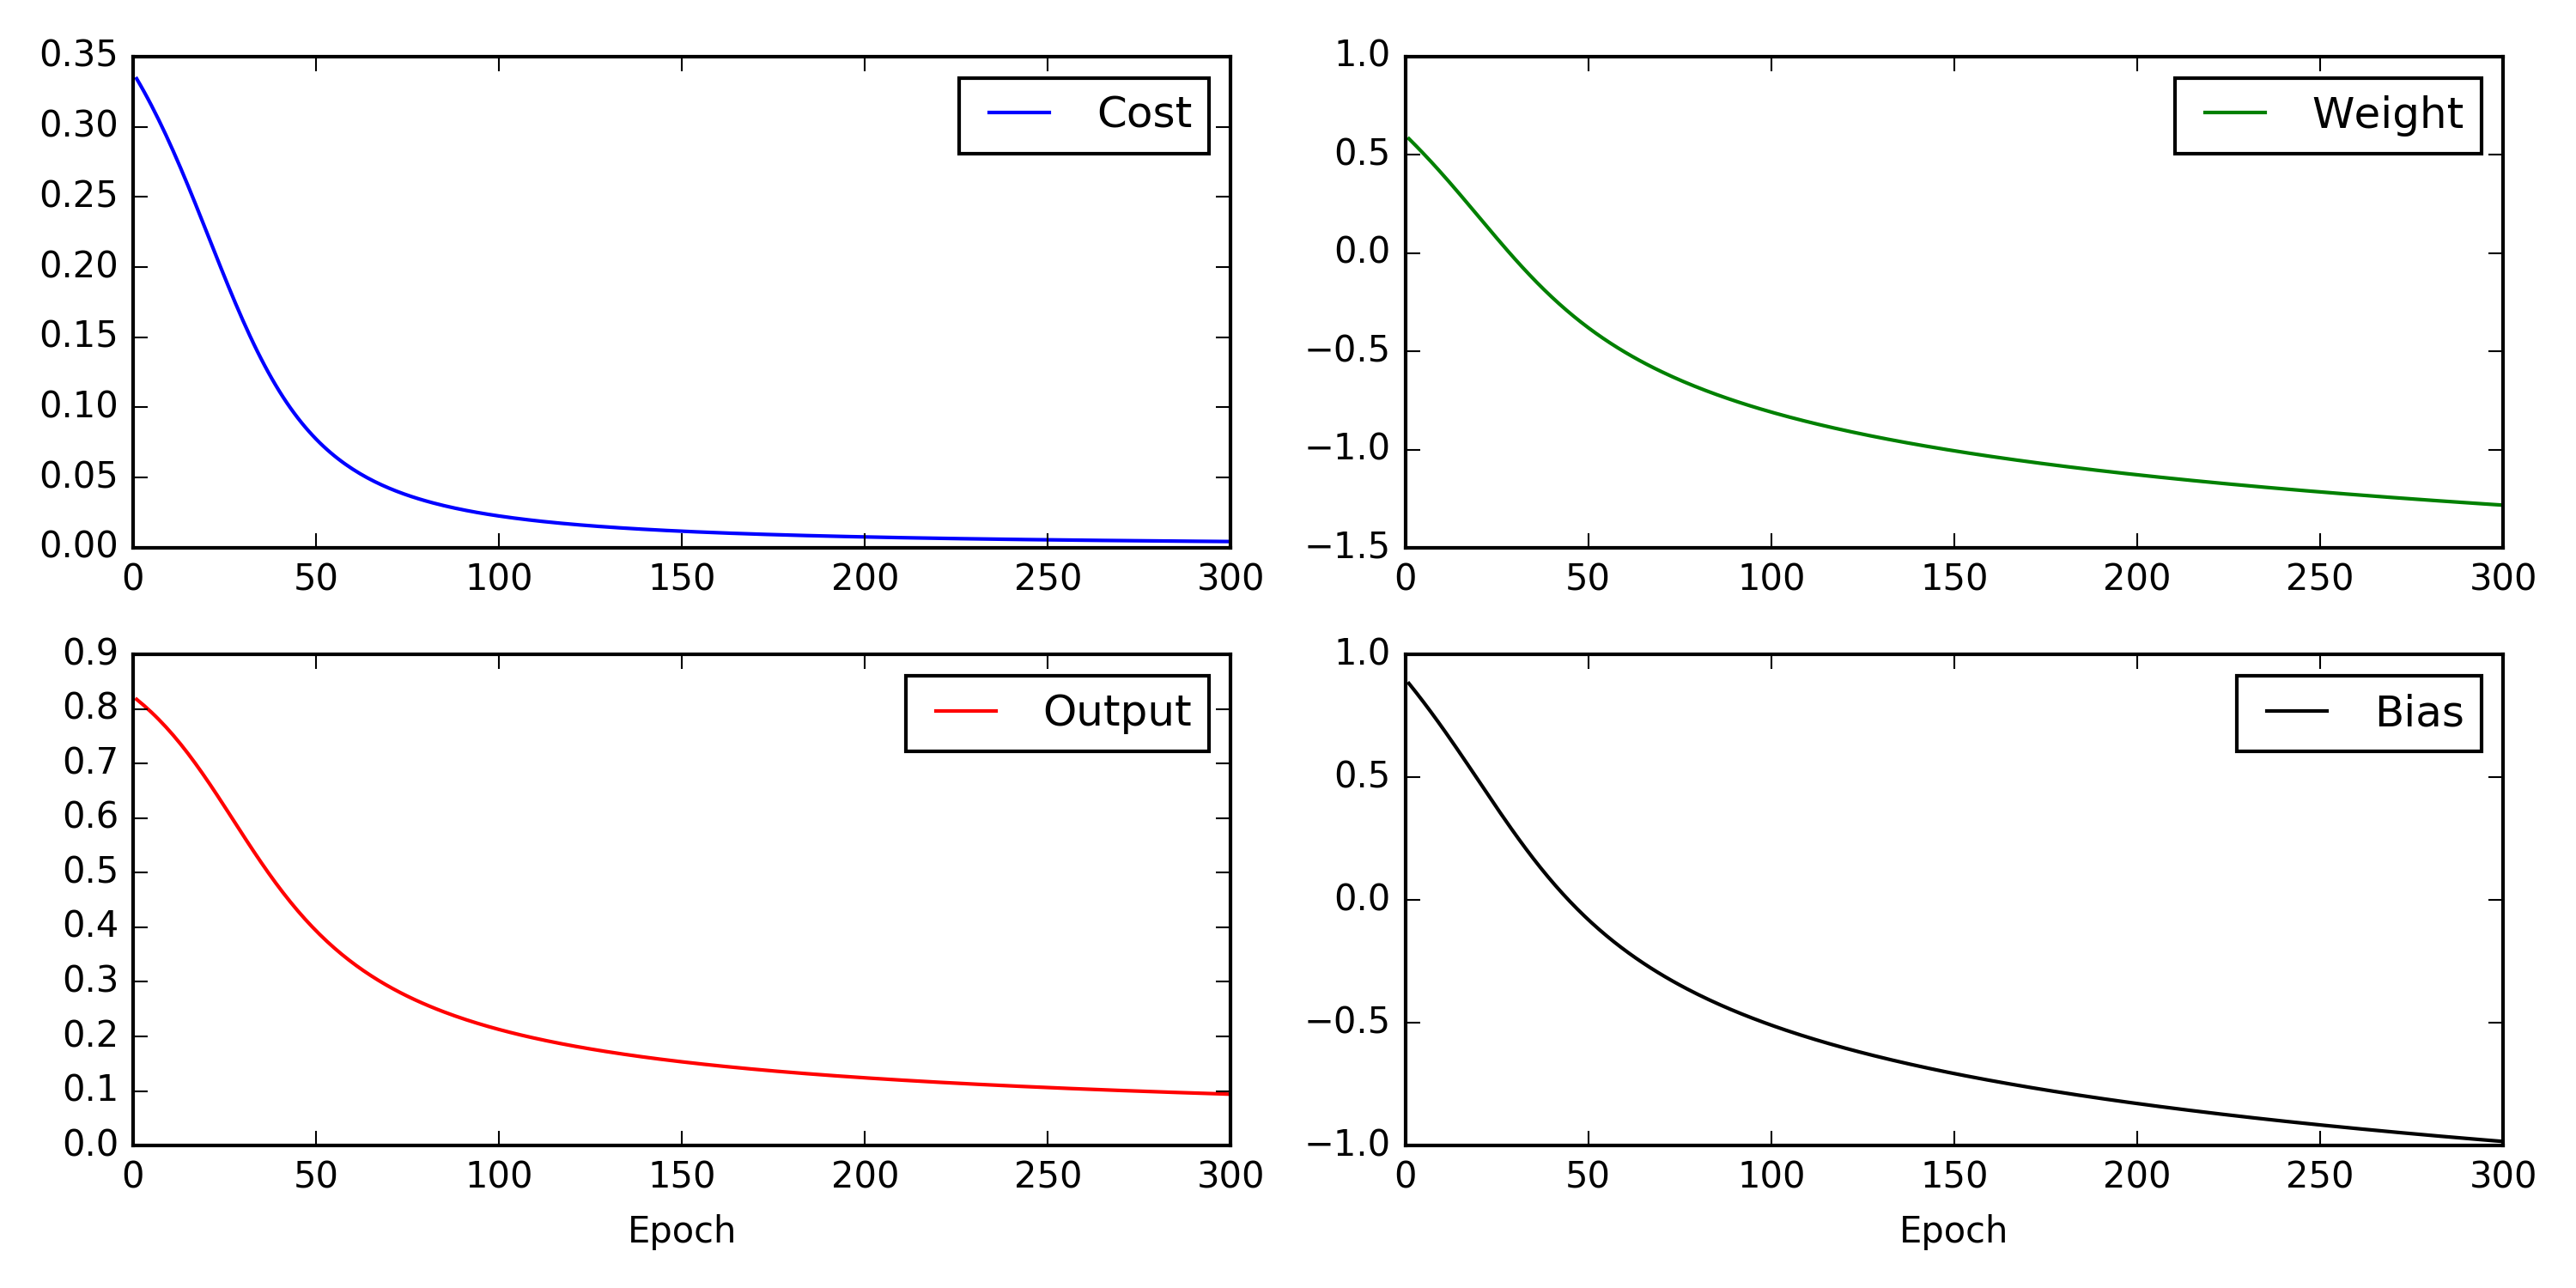
\includegraphics[width=0.75\linewidth]{./figures/ch3/animation_31}
\end{center}
As you can see, the neuron rapidly learns a weight and bias that drives down the cost, and gives an output from the neuron of about 0.09. That's not quite the desired output, 0.0, but it is pretty good. Suppose, however, that we instead choose both the starting weight and the starting bias to be 2.0. In this case the initial output is 0.98, which is very badly wrong. Let's look at how the neuron learns to output 0 in this case. %Click on ``Run'' again:
\begin{center}%
	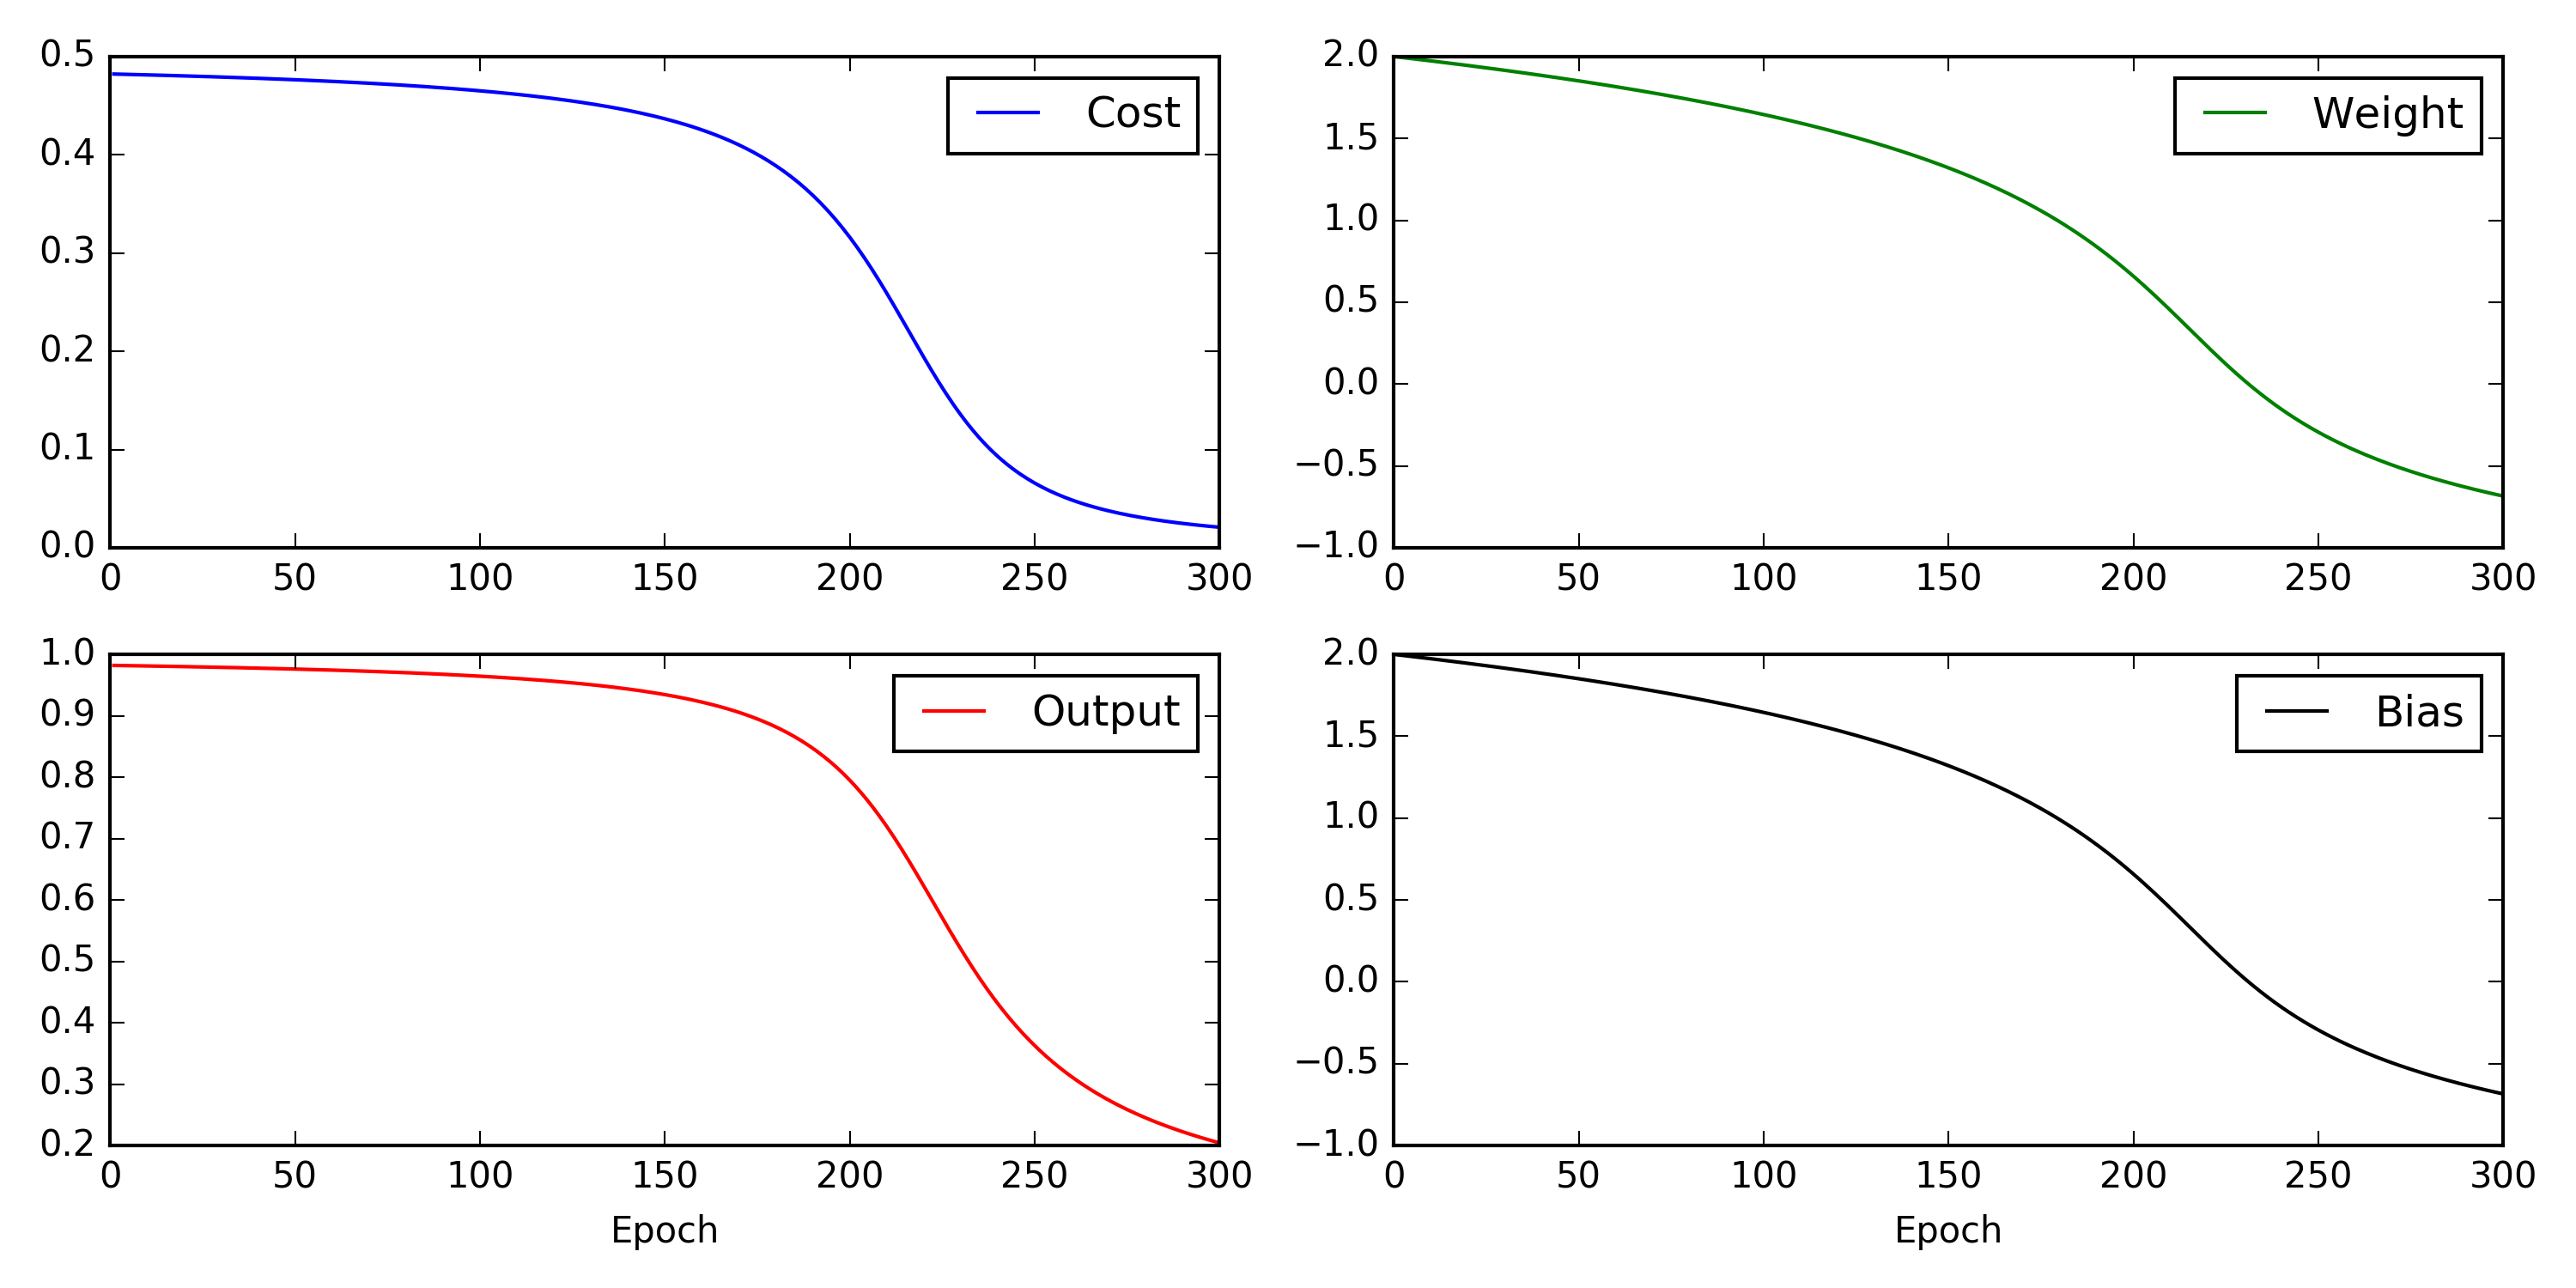
\includegraphics[width=0.75\linewidth]{./figures/ch3/animation_32}
\end{center}
Although this example uses the same learning rate ($\eta=0.15$), we can see that learning starts out much more slowly. Indeed, for the first 150 or so learning epochs, the weights and biases don't change much at all. Then the learning kicks in and, much as in our first example, the neuron's output rapidly moves closer to 0.0.

This behavior is strange when contrasted to human learning. As I said at the beginning of this section, we often learn fastest when we're badly wrong about something. But we've just seen that our artificial neuron has a lot of difficulty learning when it's badly wrong -- far more difficulty than when it's just a little wrong. What's more, it turns out that this behavior occurs not just in this toy model, but in more general networks. Why is learning so slow? And can we find a way of avoiding this slowdown?

To understand the origin of the problem, consider that our neuron learns by changing the weight and bias at a rate determined by the partial derivatives of the cost function, $\partial{}C/\partial{}w$ and $\partial{}C/\partial{}b$. So saying ``learning is slow'' is really the same as saying that those partial derivatives are small. The challenge is to understand why they are small. To understand that, let's compute the partial derivatives. Recall that we're using the quadratic cost function, which, from Equation \ref{eq:6}, is given by
\begin{equation}
C = \frac{(y-a)^2}2,\label{eq:54}
\end{equation}
where $a$ is the neuron's output when the training input $x=1$ is used, and $y=0$ is the corresponding desired output. To write this more explicitly in terms of the weight and bias, recall that $a=\sigma{}(z)$, where $z=wx+b$. Using the chain rule to differentiate with respect to the weight and bias we get
\begin{eqnarray} 
\frac{\partial C}{\partial w} & = & (a-y)\sigma'(z) x = a \sigma'(z) \label{eq:55}\\
\frac{\partial C}{\partial b} & = & (a-y)\sigma'(z) = a \sigma'(z),
\label{eq:56}
\end{eqnarray}
where I have substituted $x=1$ and $y=0$. To understand the behaviour of these expressions, let's look more closely at the $\sigma{}'(z)$ term on the right-hand side. Recall the shape of the $\sigma{}$ function:

\begin{tikzpicture}[scale=0.75]
\begin{axis}[title={Sigmoid function}]
\addplot[blue,domain=-5:5,samples=81]{1/(1+exp(-x)};
\end{axis}
\end{tikzpicture}

We can see from this graph that when the neuron's output is close to 1, the curve gets very flat, and so $\sigma{}'(z)$ gets very small. Equations \ref{eq:55} and \ref{eq:56} then tell us that $\partial{}C/\partial{}w$ and $\partial{}C/\partial{}b$ get very small. This is the origin of the learning slowdown. What's more, as we shall see a little later, the learning slowdown occurs for essentially the same reason in more general neural networks, not just the toy example we've been playing with.

\section{Introducing the cross-entropy cost function}
How can we address the learning slowdown? It turns out that we can solve the problem by replacing the quadratic cost with a different cost function, known as the cross-entropy. To understand the cross-entropy, let's move a little away from our super-simple toy model. We'll suppose instead that we're trying to train a neuron with several input variables, $x_1,x_2,\ldots$, corresponding weights $w_1,w_2,\ldots$, and a bias, $b$:
\begin{center}
	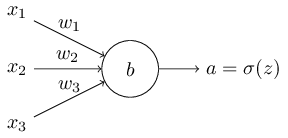
\includegraphics[scale=0.5]{./figures/ch3/tikz29}
\end{center}
The output from the neuron is, of course, $a=\sigma(z)$, where $z=\sum_jw_jb_j+b$ is the weighted sum of the inputs. We define the cross-entropy cost function for this neuron by
%C=-1n∑x[ylna+(1-y)ln(1-a)],(57)
\begin{equation}
	C = -\frac{1}{n} \sum_x \left[y \ln a + (1-y ) \ln (1-a) \right],
	\label{eq:57}
\end{equation}
where $n$ is the total number of items of training data, the sum is over all training inputs, $x$, and $y$ is the corresponding desired output.

It's not obvious that the expression (\ref{eq:57}) fixes the learning slowdown problem. In fact, frankly, it's not even obvious that it makes sense to call this a cost function! Before addressing the learning slowdown, let's see in what sense the cross-entropy can be interpreted as a cost function.

Two properties in particular make it reasonable to interpret the cross-entropy as a cost function. First, it's non-negative, that is, $C>0$. To see this, notice that: (a) all the individual terms in the sum in (\ref{eq:57}) are negative, since both logarithms are of numbers in the range 0 to 1; and (b) there is a minus sign out the front of the sum.

Second, if the neuron's actual output is close to the desired output for all training inputs, x, then the cross-entropy will be close to zero\footnote{To prove this I will need to assume that the desired outputs y are all either 0 or 1. This is usually the case when solving classification problems, for example, or when computing Boolean functions. To understand what happens when we don't make this assumption, see the exercises at the end of this section.}. To see this, suppose for example that y=0 and a≈0 for some input $x$. This is a case when the neuron is doing a good job on that input. We see that the first term in the expression (57) for the cost vanishes, since $y=0$, while the second term is just $-\ln(1-a)\approx0$. A similar analysis holds when $y=1$ and $a\approx1$. And so the contribution to the cost will be low provided the actual output is close to the desired output.

Summing up, the cross-entropy is positive, and tends toward zero as the neuron gets better at computing the desired output, $y$, for all training inputs, $x$. These are both properties we'd intuitively expect for a cost function. Indeed, both properties are also satisfied by the quadratic cost. So that's good news for the cross-entropy. But the cross-entropy cost function has the benefit that, unlike the quadratic cost, it avoids the problem of learning slowing down. To see this, let's compute the partial derivative of the cross-entropy cost with respect to the weights. We substitute $a=\sigma(z)$ into (\ref{eq:57}), and apply the chain rule twice, obtaining:
%∂C∂wj==-1n∑x(yσ(z)-(1-y)1-σ(z))∂σ∂wj-1n∑x(yσ(z)-(1-y)1-σ(z))σ′(z)xj.(58)(59)
\begin{equation}
	\frac{\partial C}{\partial w_j}  =  -\frac{1}{n} \sum_x \left(
	\frac{y }{\sigma(z)} -\frac{(1-y)}{1-\sigma(z)} \right)
	\frac{\partial \sigma}{\partial w_j} = 
 -\frac{1}{n} \sum_x \left( 
	\frac{y}{\sigma(z)} 
	-\frac{(1-y)}{1-\sigma(z)} \right)\sigma'(z) x_j.
	\label{eq:59}
\end{equation}Putting everything over a common denominator and simplifying this becomes:
\begin{equation}
	\frac{\partial C}{\partial w_j}  =  \frac{1}{n}
	\sum_x \frac{\sigma'(z) x_j}{\sigma(z) (1-\sigma(z))}
	(\sigma(z)-y).
	\label{eq:60}
\end{equation}
%∂C∂wj=1n∑xσ′(z)xjσ(z)(1-σ(z))(σ(z)-y).(60)
Using the definition of the sigmoid function, $\sigma(z)=1/(1+e^{-z})$, and a little algebra we can show that $\sigma'(z)=\sigma(z)(1-\sigma(z))$. I'll ask you to verify this in an exercise below, but for now let's accept it as given. We see that the $\sigma'(z)$ and $\sigma(z)(1-\sigma(z))$ terms cancel in the equation just above, and it simplifies to become:
%∂C∂wj=1n∑xxj(σ(z)-y).(61)
\begin{equation}
	\frac{\partial C}{\partial w_j} =  \frac{1}{n} \sum_x x_j(\sigma(z)-y).
	\label{eq:61}
\end{equation}
This is a beautiful expression. It tells us that the rate at which the weight learns is controlled by $\sigma(z)-y$, i.e., by the error in the output. The larger the error, the faster the neuron will learn. This is just what we'd intuitively expect. In particular, it avoids the learning slowdown caused by the $\sigma'(z)$ term in the analogous equation for the quadratic cost, Equation(\ref{eq:55}). When we use the cross-entropy, the $\sigma'(z)$ term gets canceled out, and we no longer need worry about it being small. This cancellation is the special miracle ensured by the cross-entropy cost function. Actually, it's not really a miracle. As we'll see later, the cross-entropy was specially chosen to have just this property.

In a similar way, we can compute the partial derivative for the bias. I won't go through all the details again, but you can easily verify that
\begin{equation}
	\frac{\partial C}{\partial b} = \frac{1}{n} \sum_x (\sigma(z)-y).
	\label{eq:62}
\end{equation}
%∂C∂b=1n∑x(σ(z)-y).(62)
Again, this avoids the learning slowdown caused by the $\sigma'(z)$ term in the analogous equation for the quadratic cost, Equation (\ref{eq:56}).
\subsection*{Exercise}
\begin{itemize}
	\item Verify that $\sigma'(z) = \sigma(z)(1-\sigma(z))$
\end{itemize}
Let's return to the toy example we played with earlier, and explore what happens when we use the cross-entropy instead of the quadratic cost. To re-orient ourselves, we'll begin with the case where the quadratic cost did just fine, with starting weight 0.6 and starting bias 0.9
%. Press "Run" to see what happens when we replace the quadratic cost by the cross-entropy
:
\begin{center}%
	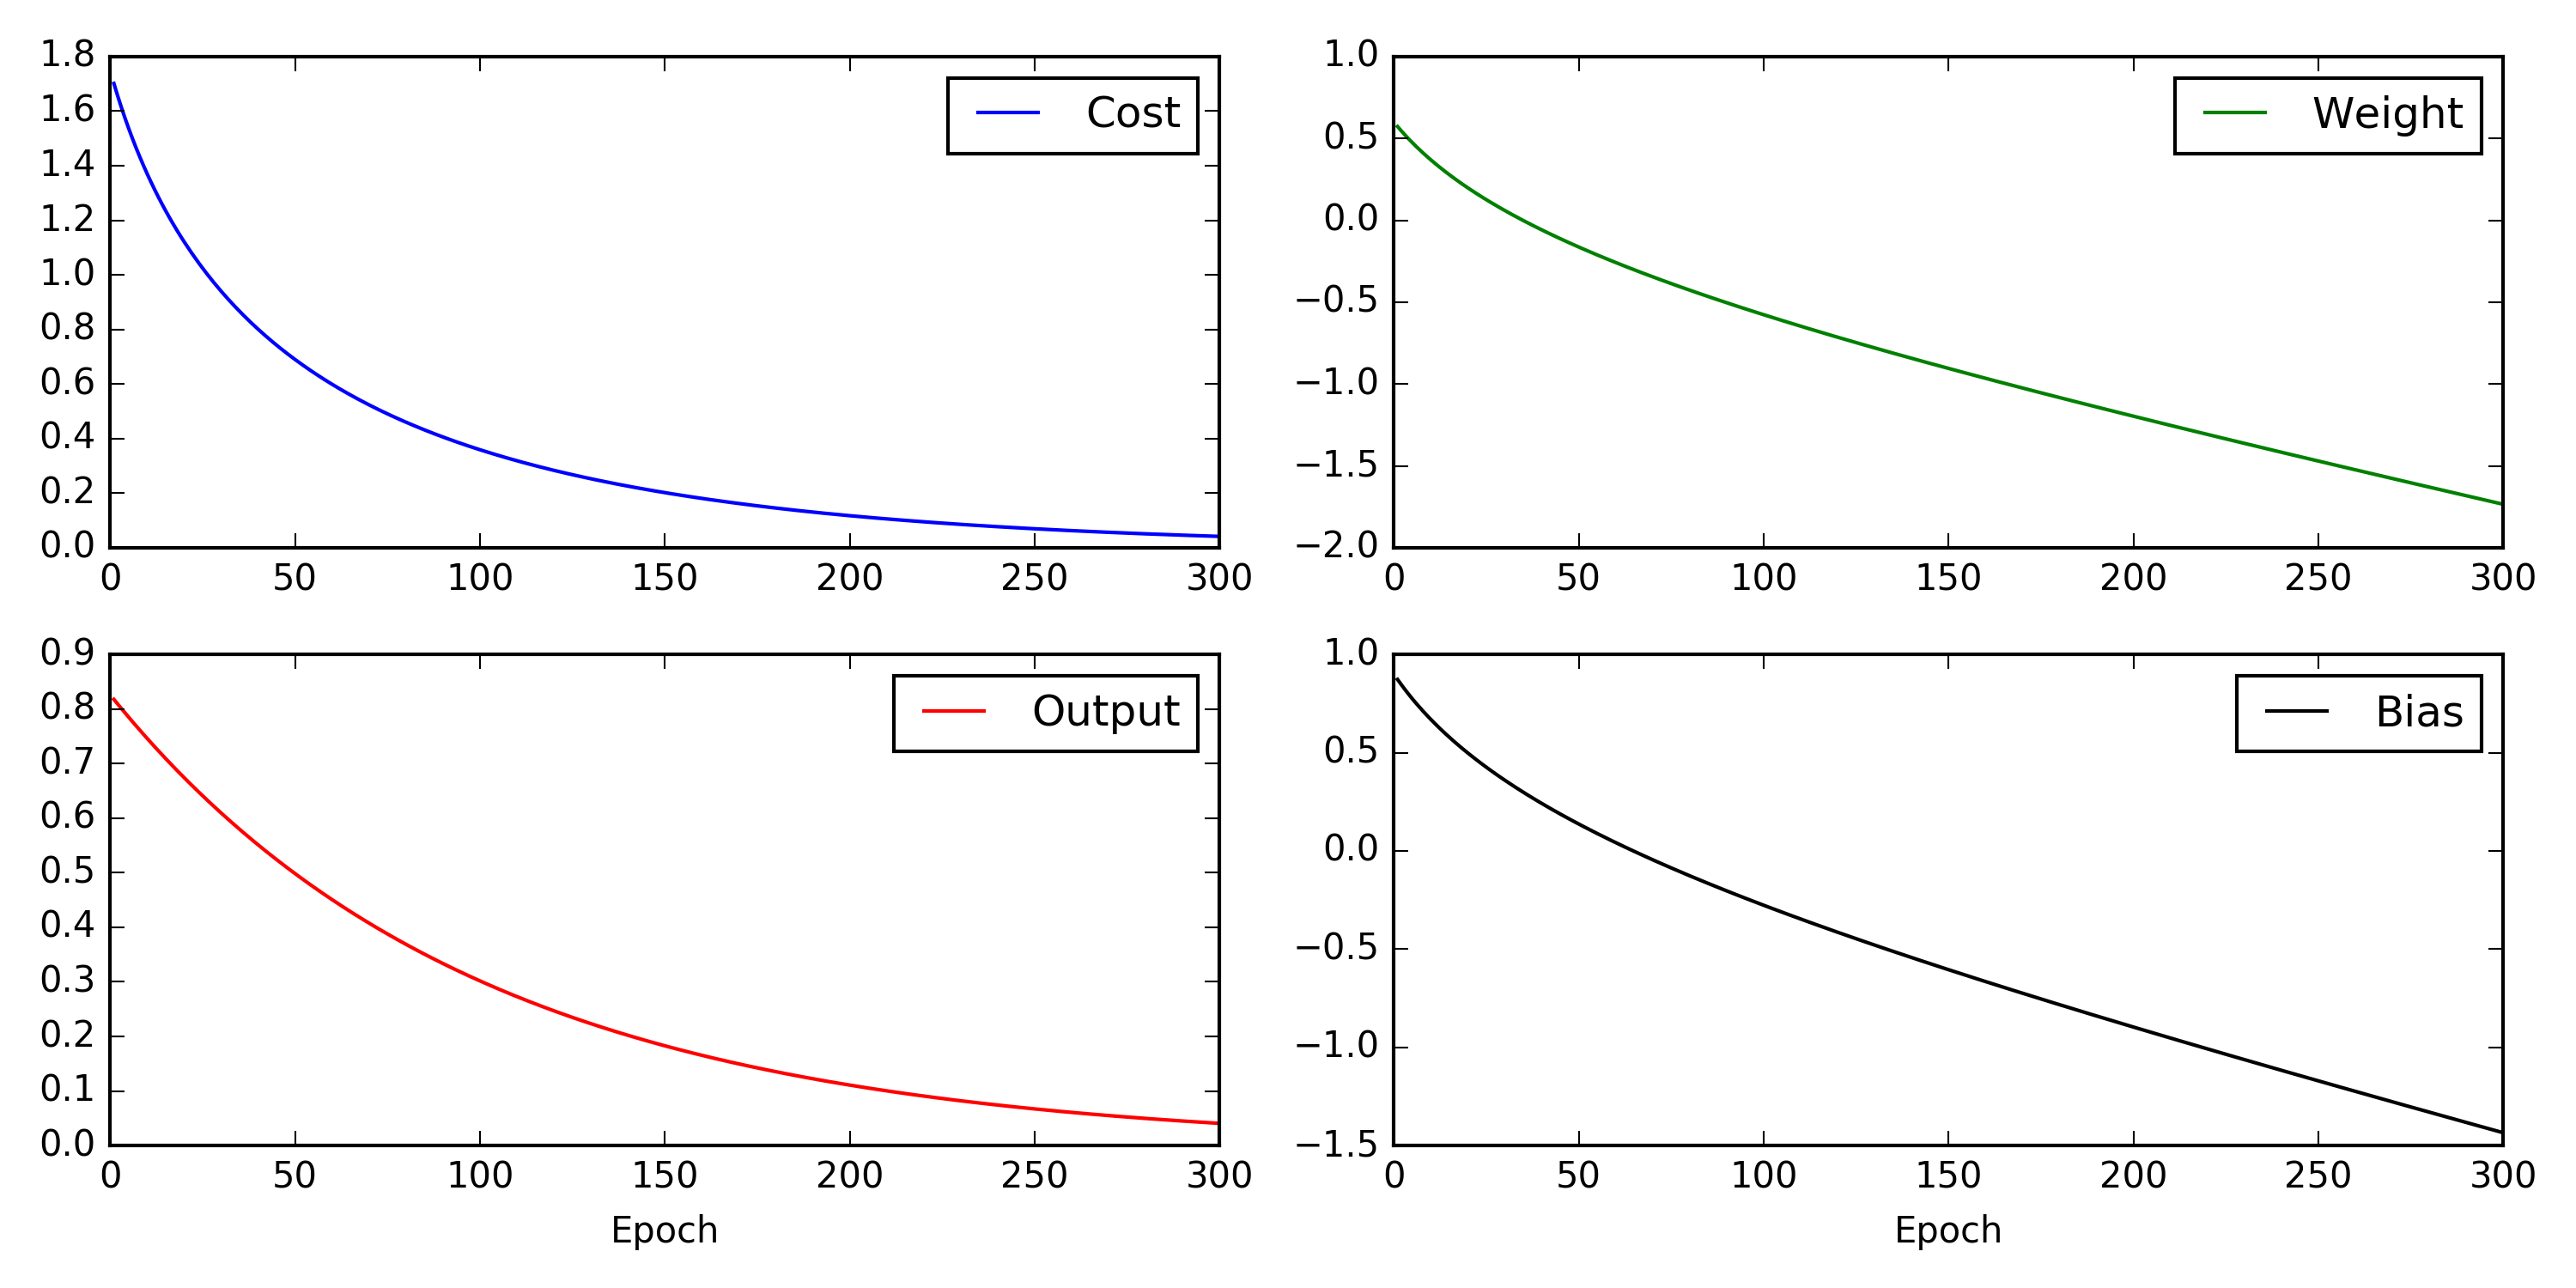
\includegraphics[width=0.75\linewidth]{./figures/ch3/animation_33}
\end{center}
Unsurprisingly, the neuron learns perfectly well in this instance, just as it did earlier. And now let's look at the case where our neuron got stuck before ([link], for comparison), with the weight and bias both starting at 2.0:
\begin{center}%
	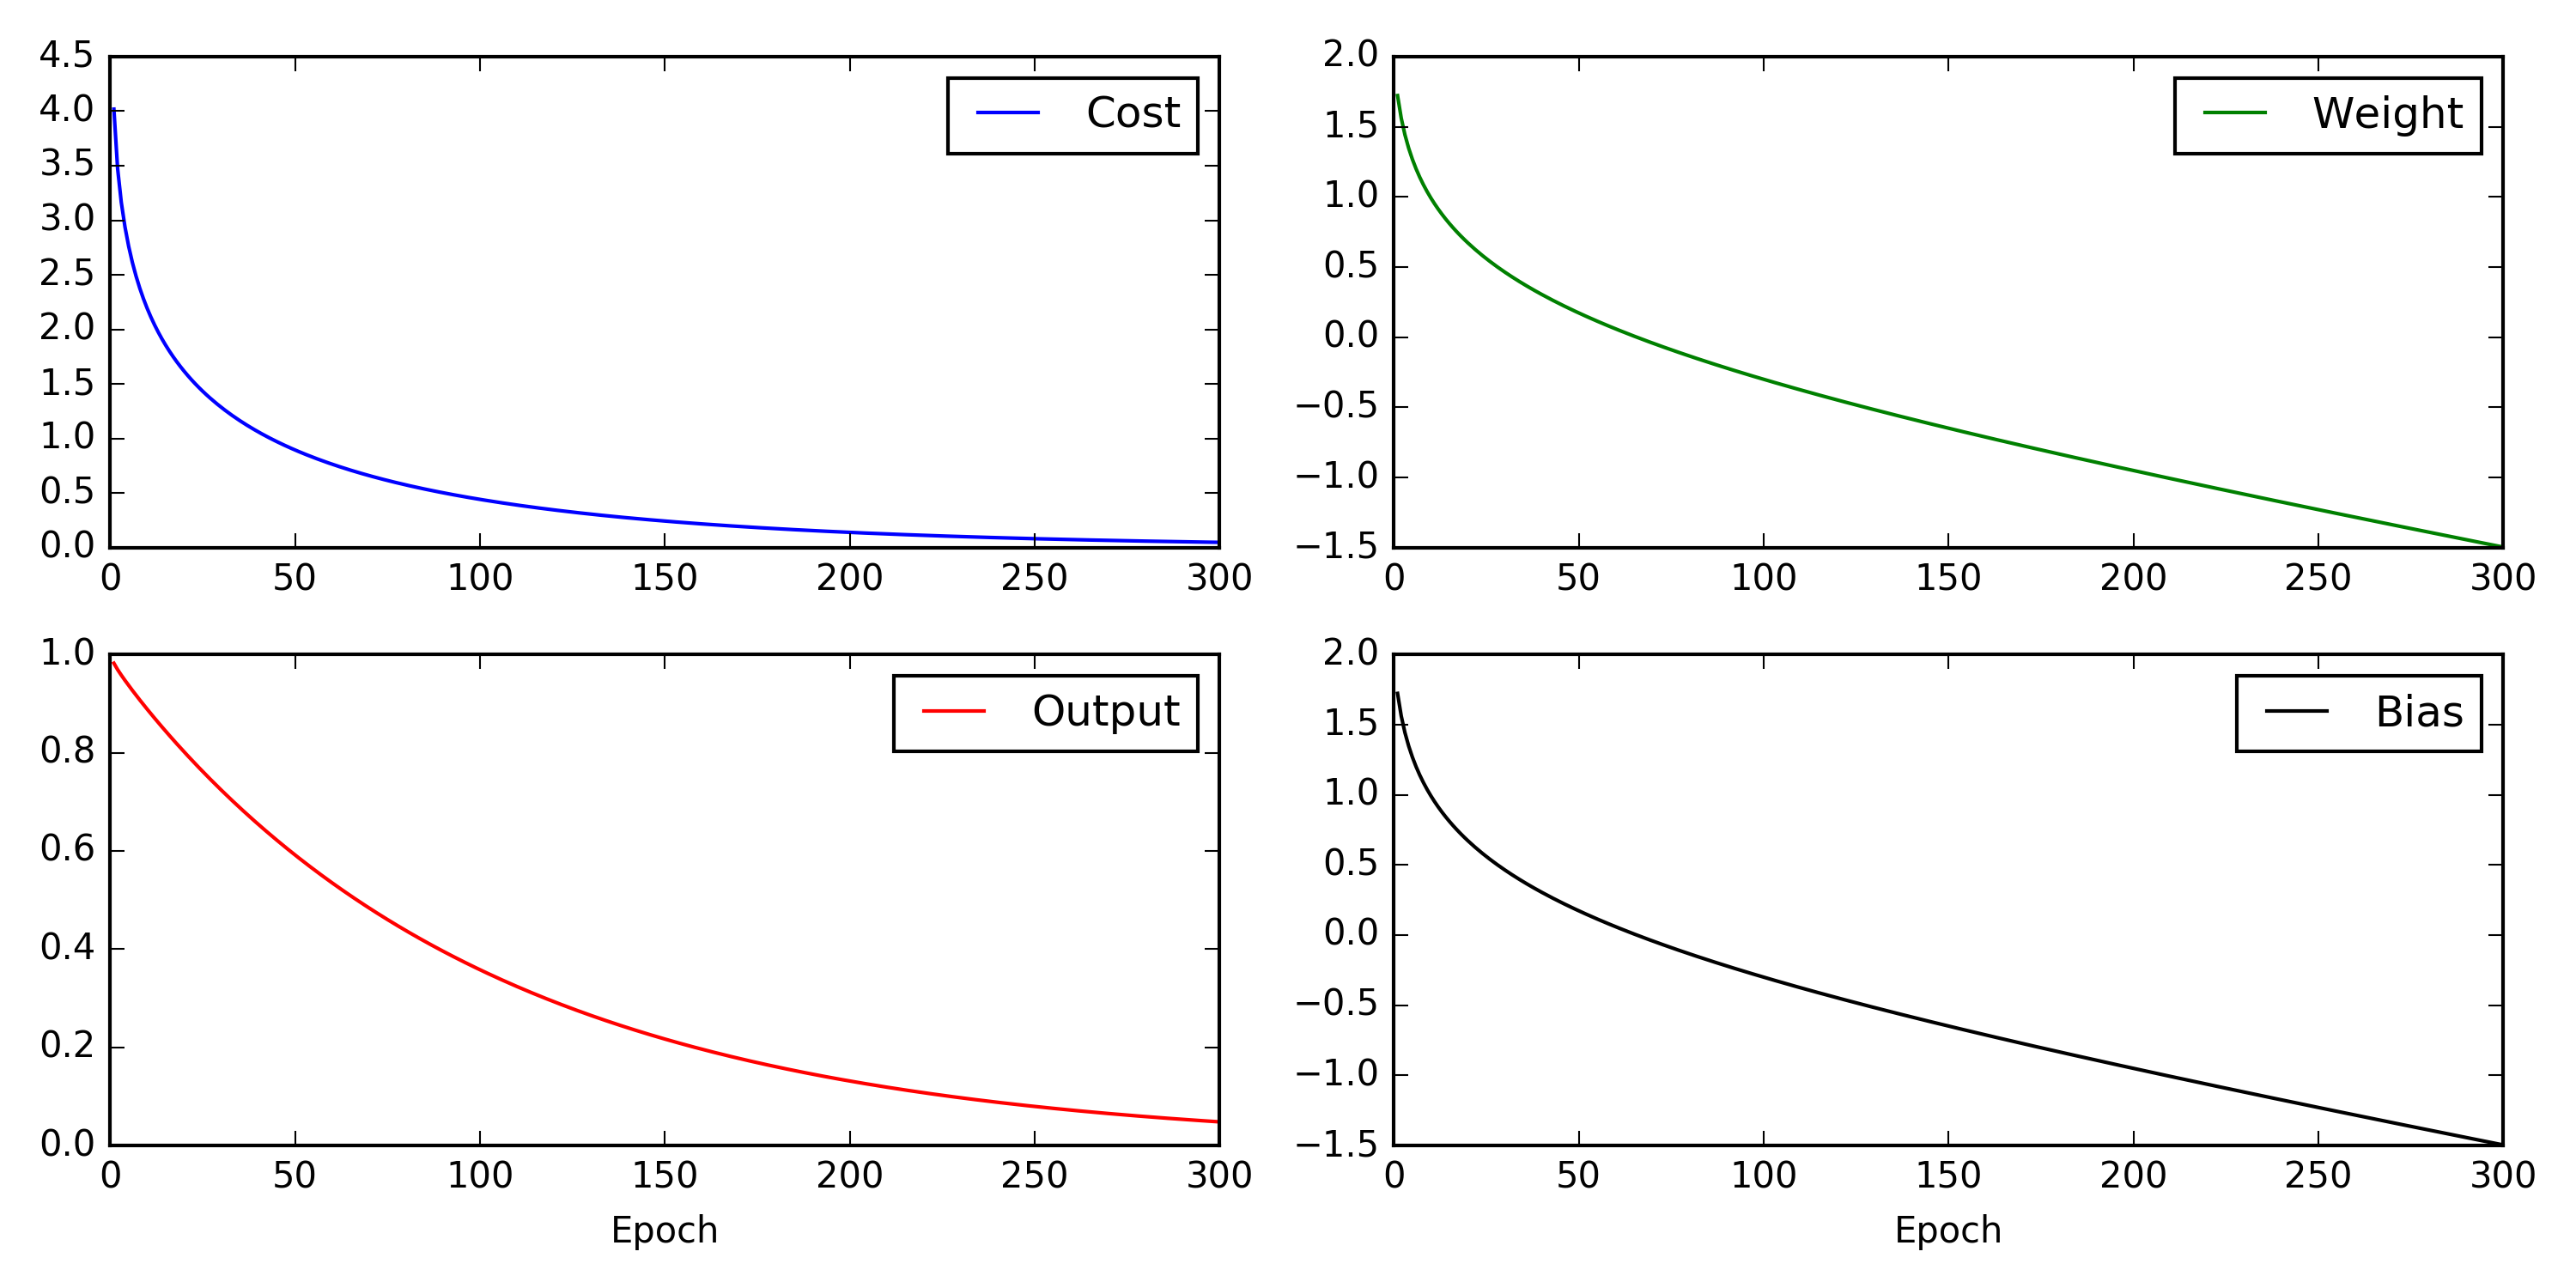
\includegraphics[width=0.75\linewidth]{./figures/ch3/animation_34}
\end{center}
Success! This time the neuron learned quickly, just as we hoped. If you observe closely you can see that the slope of the cost curve was much steeper initially than the initial flat region on the corresponding curve for the quadratic cost. It's that steepness which the cross-entropy buys us, preventing us from getting stuck just when we'd expect our neuron to learn fastest, i.e., when the neuron starts out badly wrong.

I didn't say what learning rate was used in the examples just illustrated. Earlier, with the quadratic cost, we used $\eta=0.15$. Should we have used the same learning rate in the new examples? In fact, with the change in cost function it's not possible to say precisely what it means to use the ``same'' learning rate; it's an apples and oranges comparison. For both cost functions I simply experimented to find a learning rate that made it possible to see what is going on. If you're still curious, despite my disavowal, here's the lowdown: I used $\eta=0.005$ in the examples just given.

You might object that the change in learning rate makes the graphs above meaningless. Who cares how fast the neuron learns, when our choice of learning rate was arbitrary to begin with?! That objection misses the point. The point of the graphs isn't about the absolute speed of learning. It's about how the speed of learning changes. In particular, when we use the quadratic cost learning is slower when the neuron is unambiguously wrong than it is later on, as the neuron gets closer to the correct output; while with the cross-entropy learning is faster when the neuron is unambiguously wrong. Those statements don't depend on how the learning rate is set.

We've been studying the cross-entropy for a single neuron. However, it's easy to generalize the cross-entropy to many-neuron multi-layer networks. In particular, suppose $y=y_1,y_2,\ldots$ are the desired values at the output neurons, i.e., the neurons in the final layer, while $a^L_1,a^L_2,\ldots$ are the actual output values. Then we define the cross-entropy by
%C=-1n∑x∑j[yjlna^L_j+(1-yj)ln(1-a^L_j)].(63)
\begin{equation}
	\sum_j \left[y_j \ln a^L_j + (1-y_j) \ln (1-a^L_j) \right].
	\label{eq:63}
\end{equation}
This is the same as our earlier expression, Equation (\ref{eq:57}), except now we've got the $\sum_j$ summing over all the output neurons. I won't explicitly work through a derivation, but it should be plausible that using the expression (\ref{eq:63}) avoids a learning slowdown in many-neuron networks. If you're interested, you can work through the derivation in the problem below.

Incidentally, I'm using the term ``cross-entropy'' in a way that has confused some early readers, since it superficially appears to conflict with other sources. In particular, it's common to define the cross-entropy for two probability distributions, $p_j$ and $q_j$, as $\sum_jp_j\ln{}q_j$. This definition may be connected to (\ref{eq:57}), if we treat a single sigmoid neuron as outputting a probability distribution consisting of the neuron's activation $a$ and its complement $1-a$.

However, when we have many sigmoid neurons in the final layer, the vector $a^L_j$ of activations don't usually form a probability distribution. As a result, a definition like $\sum_j p_j \ln q_j$ doesn't even make sense, since we're not working with probability distributions. Instead, you can think of (\ref{eq:63}) as a summed set of per-neuron cross-entropies, with the activation of each neuron being interpreted as part of a two-element probability distribution\footnote{Of course, in our networks there are no probabilistic elements, so they're not really probabilities.}. In this sense, (\ref{eq:63}) is a generalization of the cross-entropy for probability distributions.

When should we use the cross-entropy instead of the quadratic cost? In fact, the cross-entropy is nearly always the better choice, provided the output neurons are sigmoid neurons. To see why, consider that when we're setting up the network we usually initialize the weights and biases using some sort of randomization. It may happen that those initial choices result in the network being decisively wrong for some training input - that is, an output neuron will have saturated near 1, when it should be 0, or vice versa. If we're using the quadratic cost that will slow down learning. It won't stop learning completely, since the weights will continue learning from other training inputs, but it's obviously undesirable.

\subsection*{Exercises}
\begin{itemize}
	\item One gotcha with the cross-entropy is that it can be difficult at first to remember the respective roles of the ys and the as. It's easy to get confused about whether the right form is $$-[y \ln a + (1-y) \ln (1-a)].$$ What happens to the second of these expressions when $y=0$ or 1? Does this problem afflict the first expression? Why or why not?
	\item In the single-neuron discussion at the start of this section, I argued that the cross-entropy is small if $\sigma(z)\approx y$ for all training inputs. The argument relied on $y$ being equal to either 0 or 1. This is usually true in classification problems, but for other problems (e.g., regression problems) $y$ can sometimes take values intermediate between 0 and 1. Show that the cross-entropy is still minimized when $\sigma(z)=y$ for all training inputs. When this is the case the cross-entropy has the value:
	\begin{equation}
		C = -\frac{1}{n} \sum_x [y \ln y+(1-y) \ln(1-y)].
		\label{eq:64}
	\end{equation}
	The quantity $-[y \ln y+(1-y) \ln(1-y)]$ is sometimes known as the \textit{binary entropy}.
\end{itemize}
\subsection*{Problems}
\begin{itemize}
	\item \textbf{Many-layer multi-neuron networks} In the notation introduced in the last chapter, show that for the quadratic cost the partial derivative with respect to weights in the output layer is
	\begin{equation}
		\frac{\partial C}{\partial w^L_{jk}}  = \frac{1}{n}
		\sum_x a^{L-1}_k  (a^L_j-y_j) \sigma'(z^L_j).
		\label{eq:65}
	\end{equation}%∂C∂wLjk=1n∑xaL-1k(aLj-yj)σ′(zLj).(65)
	The term $\sigma'(z^L_j)$ causes a learning slowdown whenever an output neuron saturates on the wrong value. Show that for the cross-entropy cost the output error 
	$\delta^L$ for a single training example $x$ is given by
	\begin{equation}
		\delta^L = a^L - y.\label{eq:66}
	\end{equation}%δL=aL-y.(66)
	Use this expression to show that the partial derivative with respect to the weights in the output layer is given by
	\begin{equation}
		\frac{\partial C}{\partial w^L_{jk}}  =  \frac{1}{n} \sum_x 	a^{L-1}_k  (a^L_j-y_j).
		\label{eq:67}
	\end{equation}%∂C∂wLjk=1n∑xaL-1k(aLj-yj).(67)
	The $\sigma'(z^L_j)$ term has vanished, and so the cross-entropy avoids the problem of learning slowdown, not just when used with a single neuron, as we saw earlier, but also in many-layer multi-neuron networks. A simple variation on this analysis holds also for the biases. If this is not obvious to you, then you should work through that analysis as well.
	\item \textbf{Using the quadratic cost when we have linear neurons in the output layer} Suppose that we have a many-layer multi-neuron network. Suppose all the neurons in the final layer are linear neurons, meaning that the sigmoid activation function is not applied, and the outputs are simply $a^L_j=z^L_j$. Show that if we use the quadratic cost function then the output error $\delta^L$ for a single training example $x$ is given by
	\begin{equation}
		\delta^L = a^L-y.
		\label{eq:68}
	\end{equation}%δL=aL-y.(68)
	Similarly to the previous problem, use this expression to show that the partial derivatives with respect to the weights and biases in the output layer are given by
	\begin{eqnarray}
	\frac{\partial C}{\partial w^L_{jk}} & = & \frac{1}{n} \sum_x a^{L-1}_k  (a^L_j-y_j)\\
	\frac{\partial C}{\partial b^L_{j}} & = & \frac{1}{n} \sum_x (a^L_j-y_j).
	\label{eq:70}
	\end{eqnarray}
	%∂C∂wLjk∂C∂bLj==1n∑xaL-1k(aLj-yj)1n∑x(aLj-yj).(69)(70)
	This shows that if the output neurons are linear neurons then the quadratic cost will not give rise to any problems with a learning slowdown. In this case the quadratic cost is, in fact, an appropriate cost function to use.
\end{itemize}
\section{Using the cross-entropy to classify MNIST digits}
The cross-entropy is easy to implement as part of a program which learns using gradient descent and backpropagation. We'll do that later in the chapter, developing an improved version of our earlier program for classifying the MNIST handwritten digits, \texttt{network.py}. The new program is called \texttt{network2.py}, and incorporates not just the cross-entropy, but also several other techniques developed in this chapter\footnote{The code is available on [link]GitHub.}. For now, let's look at how well our new program classifies MNIST digits. As was the case in Chapter 1, we'll use a network with 30 hidden neurons, and we'll use a mini-batch size of 10. We set the learning rate to $\eta=0.5$\footnote{In Chapter 1 we used the quadratic cost and a learning rate of $\eta=3.0$. As discussed above, it's not possible to say precisely what it means to use the ``same'' learning rate when the cost function is changed. For both cost functions I experimented to find a learning rate that provides near-optimal performance, given the other hyper-parameter choices. \newline There is, incidentally, a very rough general heuristic for relating the learning rate for the cross-entropy and the quadratic cost. As we saw earlier, the gradient terms for the quadratic cost have an extra $\sigma' = \sigma(1-\sigma)$ term in them. Suppose we average this over values for $\sigma$, $\int_0^1\mathrm{d}\sigma \sigma(1-\sigma)=1/6$. We see that (very roughly) the quadratic cost learns an average of 6 times slower, for the same learning rate. This suggests that a reasonable starting point is to divide the learning rate for the quadratic cost by 6. Of course, this argument is far from rigorous, and shouldn't be taken too seriously. Still, it can sometimes be a useful starting point.} and we train for 30 epochs. The interface to \texttt{network2.py} is slightly different than \texttt{network.py}, but it should still be clear what is going on. You can, by the way, get documentation about \texttt{network2.py}'s interface by using commands such as \texttt{help(network2.Network.SGD)} in a Python shell.
\begin{lstlisting}
>>> import mnist_loader
>>> training_data, validation_data, test_data = mnist_loader.load_data_wrapper()
>>> import network2
>>> net = network2.Network([784, 30, 10], cost=network2.CrossEntropyCost)
>>> net.large_weight_initializer()
>>> net.SGD(training_data, 30, 10, 0.5, evaluation_data=test_data, monitor_evaluation_accuracy=True)
\end{lstlisting}	
Note, by the way, that the \texttt{net.large\_weight\_initializer()} command is used to initialize the weights and biases in the same way as described in Chapter 1. We need to run this command because later in this chapter we'll change the default weight initialization in our networks. The result from running the above sequence of commands is a network with 95.49 percent accuracy. This is pretty close to the result we obtained in Chapter 1, 95.42 percent, using the quadratic cost.
	
Let's look also at the case where we use 100 hidden neurons, the cross-entropy, and otherwise keep the parameters the same. In this case we obtain an accuracy of 96.82 percent. That's a substantial improvement over the results from Chapter 1, where we obtained a classification accuracy of 96.59 percent, using the quadratic cost. That may look like a small change, but consider that the error rate has dropped from 3.41 percent to 3.18 percent. That is, we've eliminated about one in fourteen of the original errors. That's quite a handy improvement.
	
It's encouraging that the cross-entropy cost gives us similar or better results than the quadratic cost. However, these results don't conclusively prove that the cross-entropy is a better choice. The reason is that I've put only a little effort into choosing hyper-parameters such as learning rate, mini-batch size, and so on. For the improvement to be really convincing we'd need to do a thorough job optimizing such hyper-parameters. Still, the results are encouraging, and reinforce our earlier theoretical argument that the cross-entropy is a better choice than the quadratic cost.
	
This, by the way, is part of a general pattern that we'll see through this chapter and, indeed, through much of the rest of the book. We'll develop a new technique, we'll try it out, and we'll get ``improved'' results. It is, of course, nice that we see such improvements. But the interpretation of such improvements is always problematic. They're only truly convincing if we see an improvement after putting tremendous effort into optimizing all the other hyper-parameters. That's a great deal of work, requiring lots of computing power, and we're not usually going to do such an exhaustive investigation. Instead, we'll proceed on the basis of informal tests like those done above. Still, you should keep in mind that such tests fall short of definitive proof, and remain alert to signs that the arguments are breaking down.
	
By now, we've discussed the cross-entropy at great length. Why go to so much effort when it gives only a small improvement to our MNIST results? Later in the chapter we'll see other techniques -- notably, regularization -- which give much bigger improvements. So why so much focus on cross-entropy? Part of the reason is that the cross-entropy is a widely-used cost function, and so is worth understanding well. But the more important reason is that neuron saturation is an important problem in neural nets, a problem we'll return to repeatedly throughout the book. And so I've discussed the cross-entropy at length because it's a good laboratory to begin understanding neuron saturation and how it may be addressed.

\end{document}